\chapter{A Hybrid Approach for Dysarthric Speech Recognition and Correction}

\section{\textbf{Introduction}}

Voice has become the default interface for technology, yet for millions of people, it remains unusable. Dysarthria, a motor speech disorder caused by neurological conditions such as stroke, ALS, and cerebral palsy, severely impacts articulation and intelligibility. According to Census 2011 estimates, nearly 7\% of the Indian population lives with some form of disability, with a significant portion facing speech-related impairments. Globally, tens of millions are affected, yet modern speech recognition systems continue to overlook this group.

While state-of-the-art Automatic Speech Recognition (ASR) systems such as Whisper achieve Word Error Rates (WER) below 10\% for normal speech, their performance deteriorates drastically to 30--70\% for dysarthric speech. This gap is not merely technical but deeply social, limiting accessibility to digital systems, communication tools, and assistive technologies. The challenge lies in the variability of speech patterns, lack of large-scale datasets, and sensitivity to environmental noise.

This project attempts to bridge this gap by combining data augmentation, synthetic speech generation, and semantic correction. Instead of relying solely on acoustic perfection, the system shifts focus toward understanding intent, enabling meaningful communication even when speech signals are degraded.

\begin{figure}[H]
	\centering
	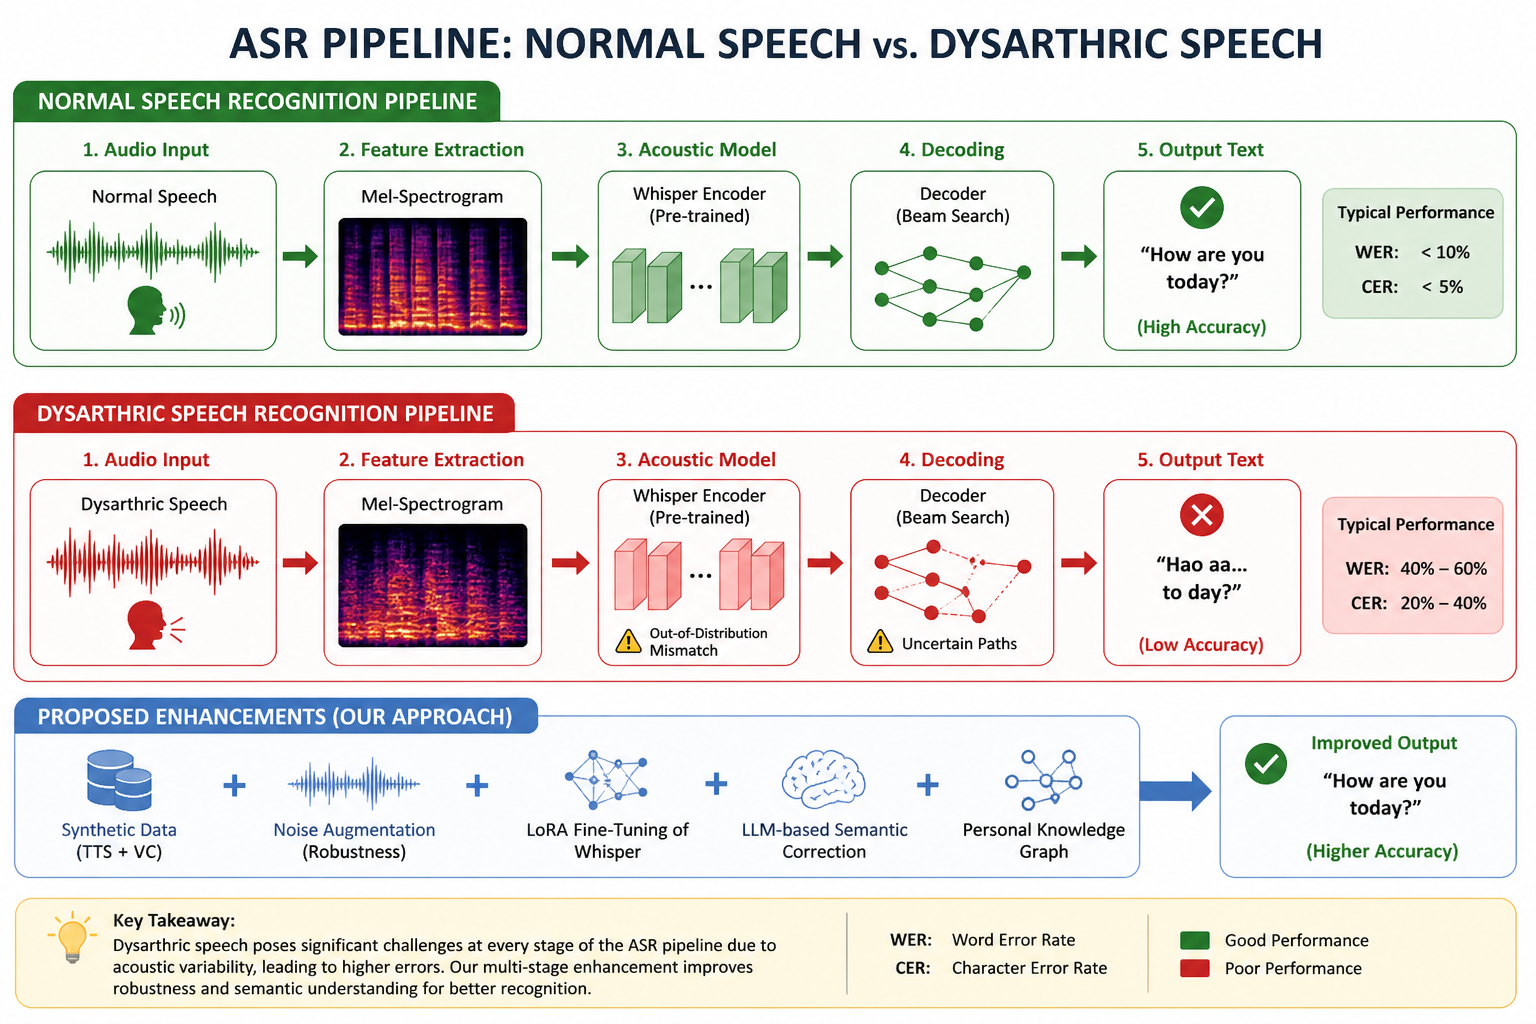
\includegraphics[width=0.8\textwidth]{Figures/asr_pipeline_vs_dysarthria.png}
	\caption{ASR Pipeline Comparison: Normal vs. Dysarthric Speech Recognition}
	\label{fig:asr_dysarthria}
\end{figure}

\section{\textbf{Literature Review}}

Recent research has explored multiple directions to improve dysarthric speech recognition. Shrestha et al. proposed a two-stage data augmentation pipeline, improving ASR performance by combining static and dynamic augmentation techniques. However, their approach struggles to generalize across patients due to high variability in speech patterns.

Vij et al. introduced a system combining CNN, Whisper, and T5 models for cerebral palsy speech detection, achieving improved classification but still suffering from low transcription accuracy. Zhang et al. proposed personalized style embeddings, enabling adaptation to individual speech patterns, but requiring sufficient speaker-specific data.

Patel et al. leveraged Mel spectrograms and transfer learning, showing improved performance, though dependent on dataset similarity. Huang et al. developed a voice conversion framework capable of generating dysarthric speech, but struggled with preserving speaker identity.

More recent approaches integrate language models. Mehta et al. demonstrated an LLM-based communication system that corrects dysarthric speech outputs, highlighting the importance of semantic understanding. Huang et al. proposed rhythm-based synthesis (DARS), improving modeling of speech patterns, though computationally intensive.

Shahamiri addressed phoneme distortions using visual spectrogram-based augmentation, achieving significant improvements for severe dysarthria. Kumar et al. generated synthetic dysarthric speech using fine-tuned TTS models, though such data often fails to capture real-world variability.

Overall, existing works focus heavily on acoustic modeling, with limited emphasis on contextual correction. Dataset scarcity, speaker variability, and lack of real-world robustness remain unresolved challenges.

\section{\textbf{Motivation}}

Despite rapid advancements in AI, accessibility for speech-impaired individuals remains limited. High ASR error rates prevent effective communication, restricting independence and digital participation. The absence of diverse datasets and personalized models further amplifies this issue.

This project is motivated by the need to build a system that not only recognizes speech but understands intent. By integrating synthetic data, noise robustness, and semantic reasoning, the system aims to provide a practical assistive solution.

\section{\textbf{Problem Statement}}

Current Automatic Speech Recognition systems perform poorly on dysarthric speech due to limited datasets, acoustic variability, and environmental noise. This results in high transcription error rates and limited accessibility of voice-based technologies for individuals with speech impairments.

\section{\textbf{Objectives}}

The objectives of the project are:
\begin{enumerate}
\item To generate synthetic dysarthric speech using Text-to-Speech (TTS) and GAN-based voice conversion techniques
\item To develop a post-ASR semantic correction layer utilizing large language models for improved transcription accuracy
\item To enhance system robustness through noise augmentation and advanced acoustic feature extraction methods
\item To integrate a Personal Knowledge Graph to support contextual speech disambiguation
\end{enumerate}

\section{\textbf{Brief Methodology of the Project}}

The proposed system follows a hybrid pipeline combining acoustic modeling and semantic reasoning. First, synthetic dysarthric speech is generated using Matcha-TTS and StarGAN-VC, increasing dataset diversity. This data is further augmented with environmental noise to simulate real-world conditions.

A frozen Whisper-v3-Turbo encoder extracts robust acoustic features from input speech. These features are mapped into the embedding space of a local large language model using a trainable projection layer. The LLM then acts as a semantic repair engine, correcting transcription errors using contextual reasoning and a Personal Knowledge Graph built from user-specific data.

This approach shifts the paradigm from pure transcription to intent-aware communication.

\section{\textbf{Assumptions and Constraints}}

\begin{itemize}
\item Availability of large-scale dysarthric speech datasets is limited
\item Synthetic speech may not fully replicate real-world speech impairments
\item Model performance depends on variability across speakers and conditions
\item Computational constraints limit full-scale training of large models
\item System evaluation is constrained by dataset diversity and noise conditions
\end{itemize}

\section{\textbf{Organization of the Report}}

This report is organized as follows:
\begin{itemize}
\item Chapter 2 discusses the fundamental concepts of speech recognition and neural models
\item Chapter 3 presents the system architecture and design methodology
\item Chapter 4 details the implementation and experimental setup
\item Chapter 5 presents results and performance evaluation using WER and CER metrics
\item Chapter 6 concludes the work and outlines future research directions
\end{itemize}